\documentclass[10pt]{article}

\usepackage[margin=0.72in]{geometry}
\usepackage{booktabs}
\usepackage{caption}
\usepackage{enumitem}
\usepackage{float}
\usepackage[T1]{fontenc}
\usepackage{graphicx}
\usepackage{hyperref}
\usepackage{microtype}
\usepackage{tabularx}
\usepackage{xcolor}

\hypersetup{
  colorlinks=true,
  linkcolor=blue!55!black,
  urlcolor=blue!55!black,
  citecolor=blue!55!black
}

\setlength{\parindent}{0pt}
\setlength{\parskip}{0.55em}
\setlength{\emergencystretch}{2em}
\setlist[itemize]{leftmargin=1.35em, itemsep=0.22em, topsep=0.25em}
\captionsetup{font=small, labelfont=bf}

\newcommand{\code}[1]{\texttt{#1}}
\newcommand{\splitkey}[1]{\texttt{#1}}

\title{\vspace{-1.2em}\textbf{DrivAerML Dataset Splits}}
\author{}
\date{}

\begin{document}
\maketitle
\vspace{-2.0em}

Deterministic train/validation/test splits for the
\href{https://huggingface.co/datasets/neashton/drivaerml}{DrivAerML} dataset
\cite{drivaerml_dataset}. The split manifest is stored at
\code{splits/manifest.json} as a flat JSON object with keys named
\code{\{split\_name\}\_\{train,val,test\}} and case IDs that match the on-disk
run directories.

DrivAerML contains 500 vehicle geometry variants at a fixed operating
condition. The public force/moment table has 484 rows; the missing 16 runs are
unavailable author-held-back cases and are excluded from all public
train/validation/test splits. The geometry-parameter table contains all 500
design rows and is used for nested data-efficiency subset selection and
image-score imputation. The \splitkey{geometry} split itself uses sampled
STL-surface Chamfer distances to measure how different each public geometry is
from its neighbors.

\section*{Splits at a glance}

\begin{tabularx}{\textwidth}{@{}l l r r r X@{}}
\toprule
Split & Type & Train & Val & Test & What it tests \\
\midrule
\splitkey{full} & In-dist & 400 & 34 & 50 & Seed-42 random public baseline split \\
\splitkey{medium} & In-dist & 133 & 34 & 50 & Data efficiency, 1/3 of \splitkey{full} training data \\
\splitkey{scarce} & In-dist & 67 & 34 & 50 & Data efficiency, 1/6 of \splitkey{full} training data \\
\splitkey{super\_scarce} & In-dist & 11 & 34 & 50 & Extreme data efficiency, 1/36 of \splitkey{full} training data \\
\splitkey{geometry} & OOD & 339 & 48 & 97 & STL-surface Chamfer extrapolation using the top 20\% local-isolation distance \\
\splitkey{high\_drag} & OOD & 339 & 48 & 97 & High-drag extrapolation using the top 20\% \code{cd} \\
\splitkey{low\_drag} & OOD & 339 & 48 & 97 & Low-drag extrapolation using the bottom 20\% \code{cd} \\
\splitkey{rear\_separation} & OOD & 339 & 48 & 97 & Image-derived low-speed wake and rear-separation extent \\
\bottomrule
\end{tabularx}

\textbf{Difficulty ladders:}
\begin{itemize}
  \item Data efficiency: \splitkey{full} < \splitkey{medium} < \splitkey{scarce} < \splitkey{super\_scarce}, with fixed validation/test sets.
  \item OOD physics: \splitkey{geometry}, \splitkey{high\_drag}, \splitkey{low\_drag}, and \splitkey{rear\_separation}.
\end{itemize}

\section*{Which split should I use?}

\begin{itemize}
  \item \textbf{Simple baseline or literature compatibility}: \splitkey{full}
  \item \textbf{Data efficiency study}: compare \splitkey{super\_scarce}, \splitkey{scarce}, \splitkey{medium}, and \splitkey{full}
  \item \textbf{Geometry extrapolation}: \splitkey{geometry}
  \item \textbf{Image-observed rear-separation regimes}: \splitkey{rear\_separation}
  \item \textbf{Targeted coefficient extrapolation}: \splitkey{high\_drag} or \splitkey{low\_drag}
\end{itemize}

\section*{Using the committed splits}

For standard benchmark use, consume the committed manifest at
\code{splits/manifest.json}; no regeneration is required. The manifest is the
source of truth for all split membership and contains one train, validation,
and test key for each split listed above.

\begin{verbatim}
import json
from pathlib import Path

manifest = json.loads(Path("splits/manifest.json").read_text())

train_ids = manifest["geometry_train"]
val_ids = manifest["geometry_val"]
test_ids = manifest["geometry_test"]
\end{verbatim}

Change the \code{geometry} prefix to \code{full}, \code{medium},
\code{scarce}, \code{super\_scarce}, \code{high\_drag}, \code{low\_drag}, or
\code{rear\_separation} to select a different split. Each value is a sorted
list of \code{run\_N} directory names. The manifest already excludes the 16
unavailable held-back cases, so users should not filter those IDs again unless
their local dataset copy is incomplete.

\section*{Design principles}

\begin{itemize}
  \item \textbf{Validation is always in-distribution with train.} For OOD splits, the validation set is drawn from the training-side population, not from the extreme OOD test region.
  \item \textbf{Keep the public baseline stable.} \splitkey{full} is a seed-42 random public split: 400 train, 34 validation, 50 test, with the 16 unavailable cases excluded.
  \item \textbf{Use direct surface distances for geometry OOD.} \splitkey{geometry} ranks public STL surfaces by nearest-neighbor Chamfer isolation, which is a stronger geometry-difference signal than parameter-space distance alone.
  \item \textbf{Use the dataset metadata directly where it defines the split axis.} Force-regime splits are generated from \code{force\_mom\_all.csv}. The \splitkey{geometry} split is generated from STL-surface Chamfer scores in \code{chamfer\_metrics.csv}; \code{geo\_parameters\_all.csv} supports the nested data-efficiency subsets and image-score imputation.
  \item \textbf{Use flow images as physics labels.} The retained image-derived split scores low-speed recirculation/separation extent from centreline and near-rear velocity-magnitude PNGs.
  \item \textbf{Represent DrivAerML physics.} The retained OOD axes target surface-shape novelty, high- and low-drag regimes, and visible rear-separation flow structure.
  \item \textbf{Nested data-efficiency subsets.} \splitkey{super\_scarce\_train} is a strict subset of \splitkey{scarce\_train}, \splitkey{scarce\_train} is a strict subset of \splitkey{medium\_train}, and \splitkey{medium\_train} is a strict subset of \splitkey{full\_train}.
  \item \textbf{Test set integrity.} Test cases should not be used for hyperparameter tuning, model selection, normalization fitting, or visual inspection-driven iteration.
\end{itemize}

\section*{Split details}

\subsection*{\splitkey{full}}

The default public split is a seeded random split over run IDs, not a
physics-stratified split. It constructs \code{torch.randperm(500)} with seed
42, shifts the IDs to \code{1..500}, removes the 16 unavailable hidden cases,
then assigns the first 400 public IDs to train, the next 50 to test, and the
remaining 34 to validation. The case IDs are sorted before being stored in the
manifest. For reference, these IDs match the public
\href{https://github.com/Emmi-AI/noether/blob/main/src/noether/data/datasets/cfd/caeml/drivaerml/split.py}{DrivAerMLDefaultSplitIDs}
implementation in Noether \cite{noether_split}.

\subsection*{\splitkey{medium}, \splitkey{scarce}, and \splitkey{super\_scarce}}

Same validation/test as \splitkey{full}, but the training set is a nested
force- and geometry-diverse subset of \splitkey{full\_train}: 133 cases for
\splitkey{medium}, 67 cases for \splitkey{scarce}, and 11 cases for
\splitkey{super\_scarce}. The subset order is a greedy max-min selection in
standardized force/geometry feature space using \code{cd}, \code{cl},
\code{cs}, and all public geometry parameters.

By construction, \splitkey{super\_scarce\_train} is a subset of
\splitkey{scarce\_train}, \splitkey{scarce\_train} is a subset of
\splitkey{medium\_train}, and \splitkey{medium\_train} is a subset of
\splitkey{full\_train}.

\subsection*{\splitkey{geometry}}

The preferred geometry OOD split when STL-derived geometry metrics are
available. It uses \code{chamfer\_metrics.csv}, where each public run is
represented by deterministic surface samples from its STL mesh. The committed
metrics were generated with 10,000 surface samples per public run, seed 42, no
recentering, global median bounding-box scaling, and symmetric Chamfer RMS
distances.

The split uses \code{ood\_score}, currently the mean distance to the 10 nearest
neighboring public geometries:

\begin{verbatim}
geometry_score_i = mean_10_nearest_neighbors(chamfer_distance_i)
\end{verbatim}

The top 20\% of public runs by this local-isolation score form the OOD test
set. Validation is sampled from the remaining training-side pool:

\begin{verbatim}
geometry_test  = top_20_percent_i(geometry_score_i)
geometry_pool  = public_runs - geometry_test
geometry_val   = deterministic_random_sample(geometry_pool, round(0.125 * |geometry_pool|))
geometry_train = geometry_pool - geometry_val
\end{verbatim}

This split captures surface-level differences that may not dominate
standardized parameter distances. In the current Chamfer metrics, the most
locally isolated public geometries include \splitkey{run\_393},
\splitkey{run\_65}, \splitkey{run\_129}, \splitkey{run\_293},
\splitkey{run\_439}, \splitkey{run\_345}, \splitkey{run\_495}, and
\splitkey{run\_237}. Figure~\ref{fig:force_geometry} shows the geometry split
both against \code{Cd} and against the Chamfer score used to define the
holdout, and Figure~\ref{fig:geometry_examples} shows complete-car examples
from the low-score training side and high-score geometry-test side, including a
same-crop transparent overlay.

\subsection*{\splitkey{high\_drag} and \splitkey{low\_drag}}

Both splits sort public cases by drag coefficient \code{cd}.
\splitkey{high\_drag} holds out the top 20\% by \code{cd};
\splitkey{low\_drag} holds out the bottom 20\% by \code{cd}. In both cases,
train/validation are sampled from the complementary 80\% so validation remains
in-distribution with training. Figure~\ref{fig:force_geometry} shows these
holdouts across run IDs.

In the current CSV, the highest-drag public runs include \splitkey{run\_115},
\splitkey{run\_39}, \splitkey{run\_29}, \splitkey{run\_186}, and
\splitkey{run\_226}. The lowest-drag public runs include \splitkey{run\_289},
\splitkey{run\_159}, \splitkey{run\_10}, \splitkey{run\_345}, and
\splitkey{run\_426}.

\begin{figure}[H]
  \centering
  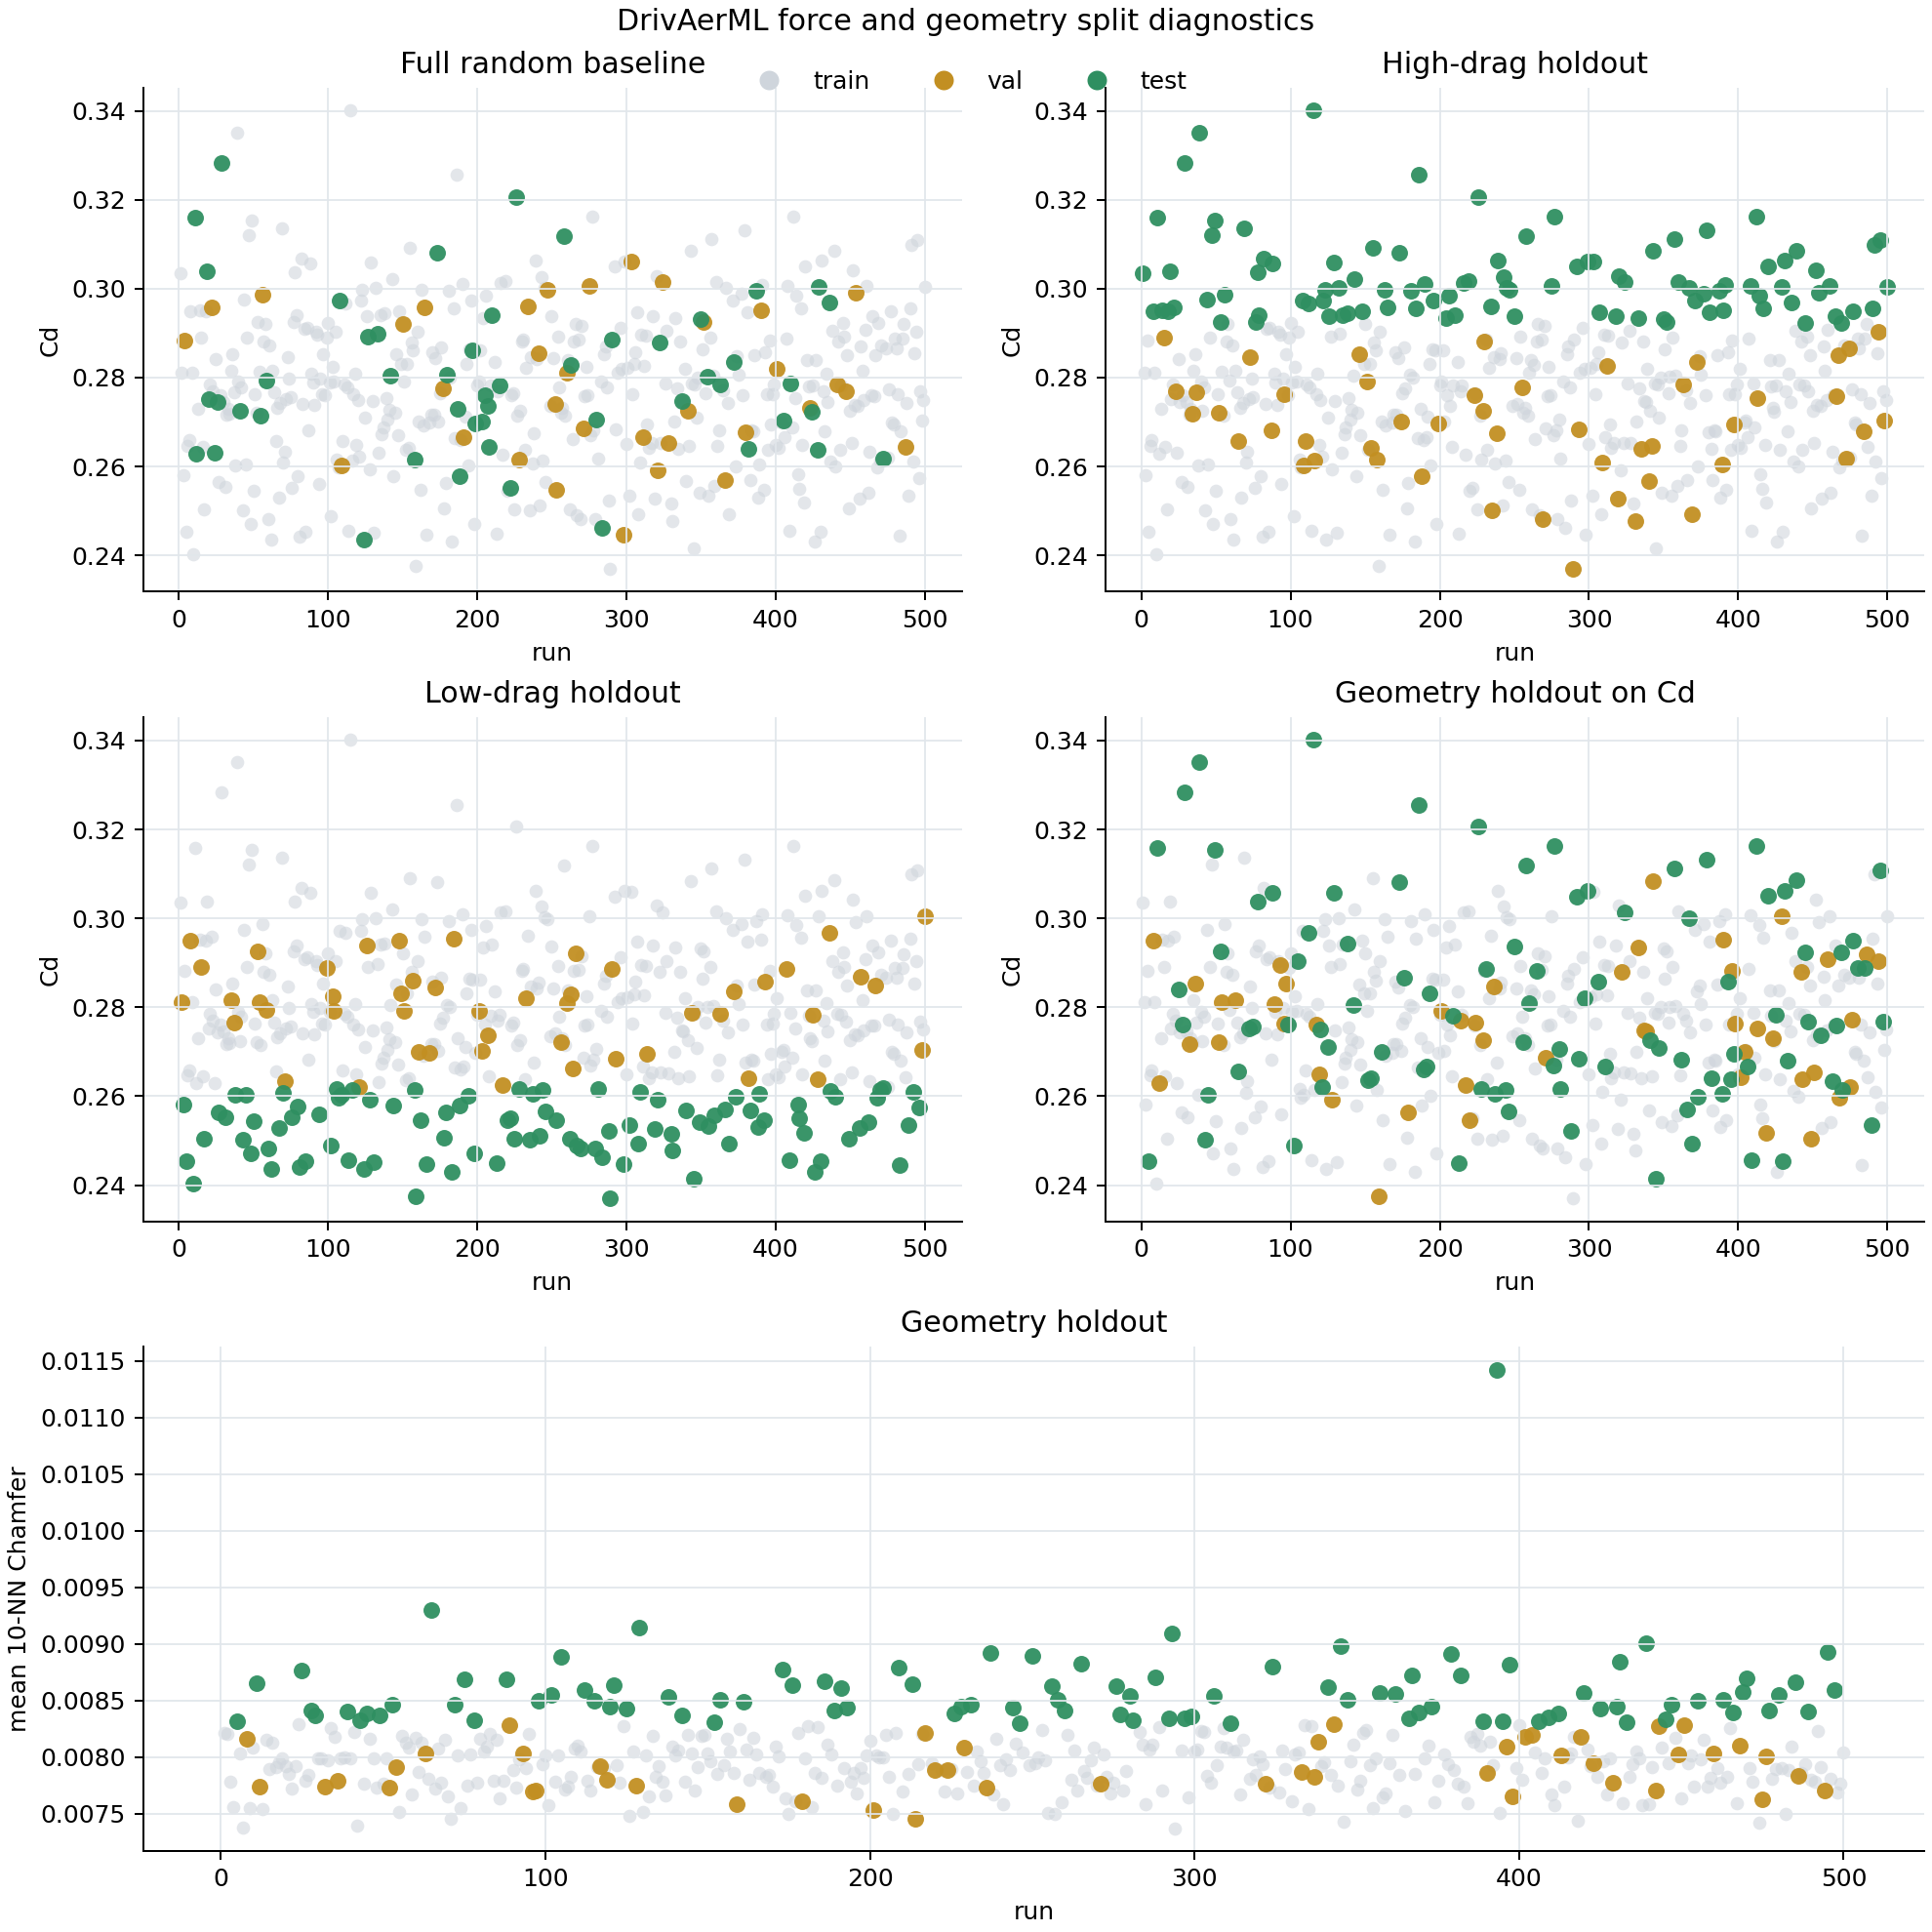
\includegraphics[width=0.96\textwidth]{force_regimes.png}
  \caption{Force and geometry split diagnostics. The panels show the full random baseline, high-drag holdout, low-drag holdout, geometry holdout on \code{Cd}, and geometry holdout on STL-surface Chamfer score. The x-axis is run ID, and points are colored by each split's train, validation, and test partitions.}
  \label{fig:force_geometry}
\end{figure}

\begin{figure}[H]
  \centering
  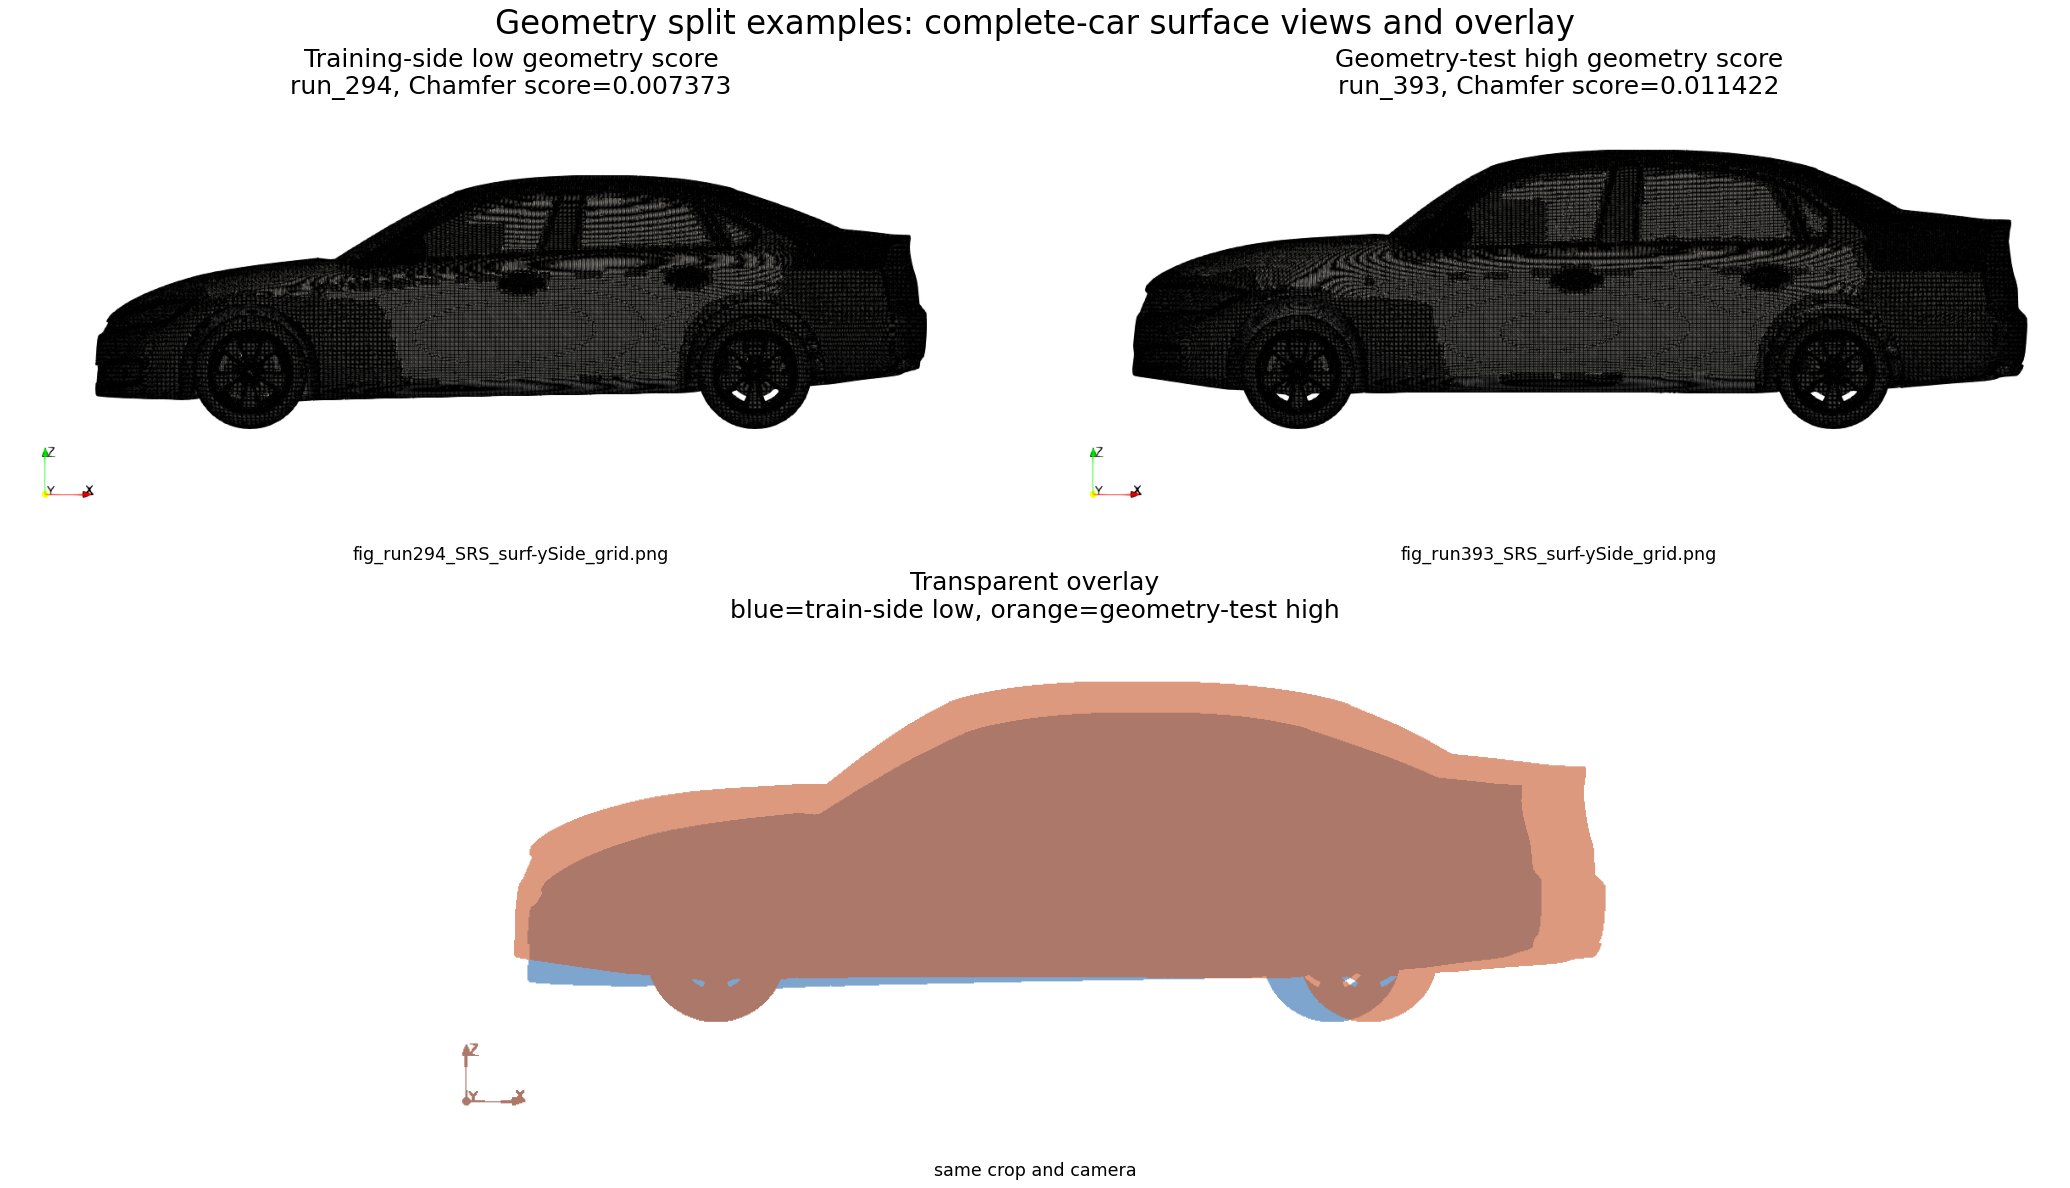
\includegraphics[width=\textwidth]{geometry_split_examples.png}
  \caption{Geometry split examples. The low-score training-side case is \splitkey{run\_294} (\code{geometry\_score=0.007373}, \code{Cd=0.281193}, \code{Cl=-0.017952}), and the high-score geometry-test case is \splitkey{run\_393} (\code{geometry\_score=0.011422}, \code{Cd=0.285732}, \code{Cl=0.052227}). The bottom panel overlays the same-crop side views with \splitkey{run\_294} in blue and \splitkey{run\_393} in orange.}
  \label{fig:geometry_examples}
\end{figure}

\subsection*{Image-derived flow-regime split}

The image-derived split is intended to capture a visible flow-physics regime
that is not fully described by high or low integrated coefficients. It uses
selected PNG diagnostics from each \code{run\_*/images/} folder, and
Figure~\ref{fig:image_regime} shows the resulting rear-separation score
distribution plus the same train/validation/test membership against \code{Cd}:

\begin{itemize}
  \item \splitkey{rear\_separation}: low-speed wake area from the \code{y=0} centreline velocity-magnitude PNG and seven near-rear \code{xNormal} velocity-magnitude PNGs (\code{p43000} through \code{p55000}).
\end{itemize}

The score estimates recirculation/separation size by counting the low-speed
blue/cyan/green part of the fixed \code{|U|/U0} colormap. The committed score
combines 60\% centreline wake area with 40\% mean near-rear \code{xNormal}
low-speed area.

For this score, the top 20\% of public runs are held out as test. Validation is
sampled from the remaining 80\%.

\begin{figure}[H]
  \centering
  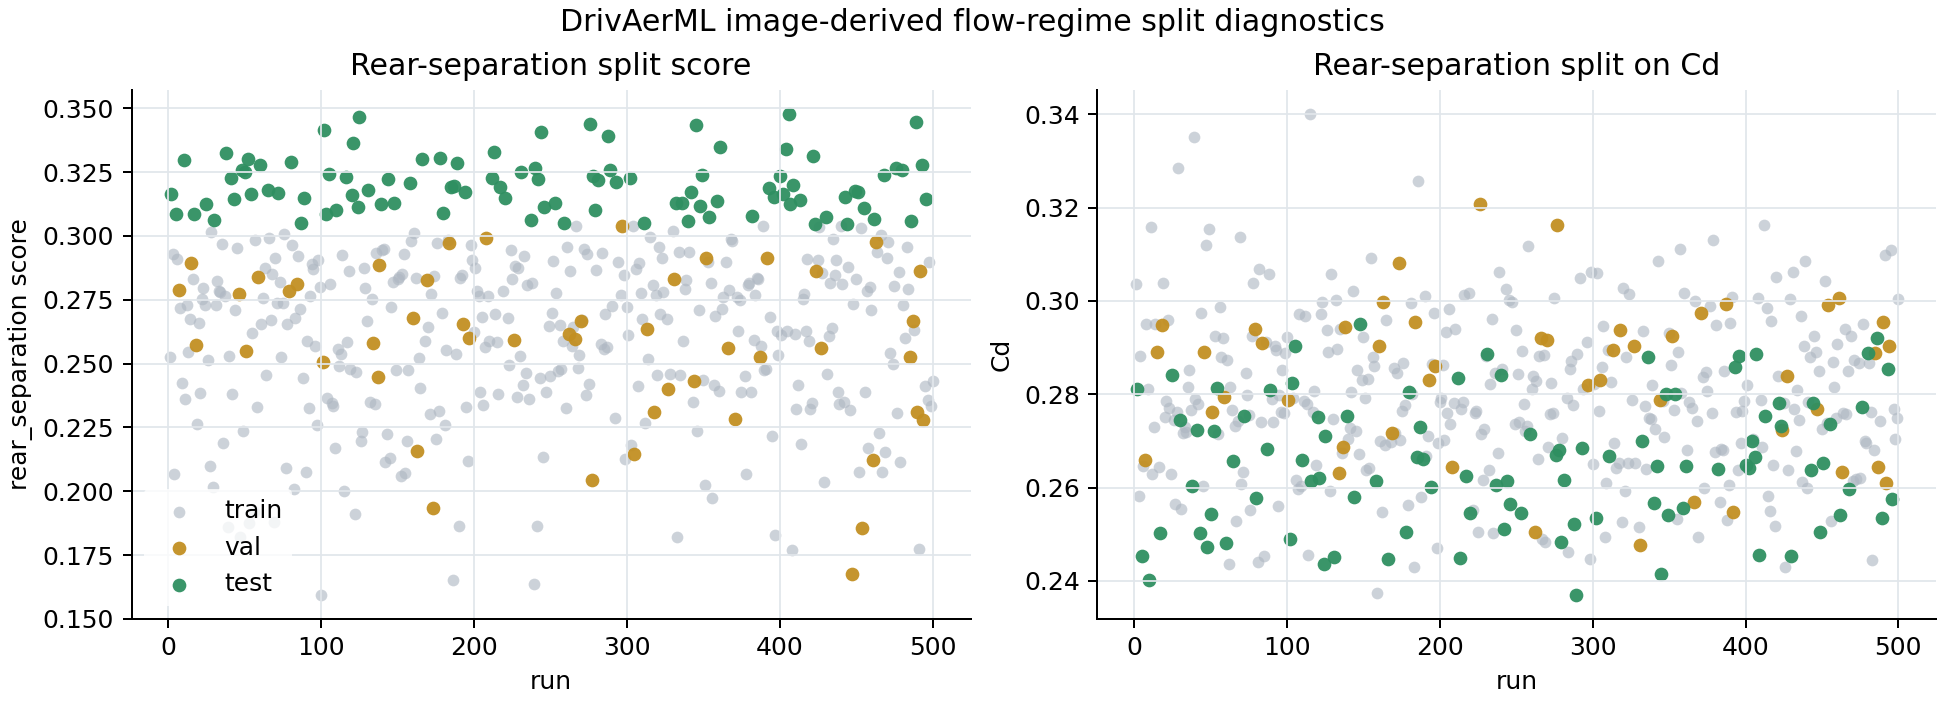
\includegraphics[width=0.96\textwidth]{image_regimes.png}
  \caption{Image-derived rear-separation split diagnostics. The left panel shows the rear-separation score used for the holdout, and the right panel shows \code{Cd} for the same \splitkey{rear\_separation\_train}, \splitkey{rear\_separation\_val}, and \splitkey{rear\_separation\_test} partitions.}
  \label{fig:image_regime}
\end{figure}

Figure~\ref{fig:image_examples} shows centreline \code{y=0}
velocity-magnitude slices for observed low-score and high-score cases from the
image-derived metric.

\begin{figure}[H]
  \centering
  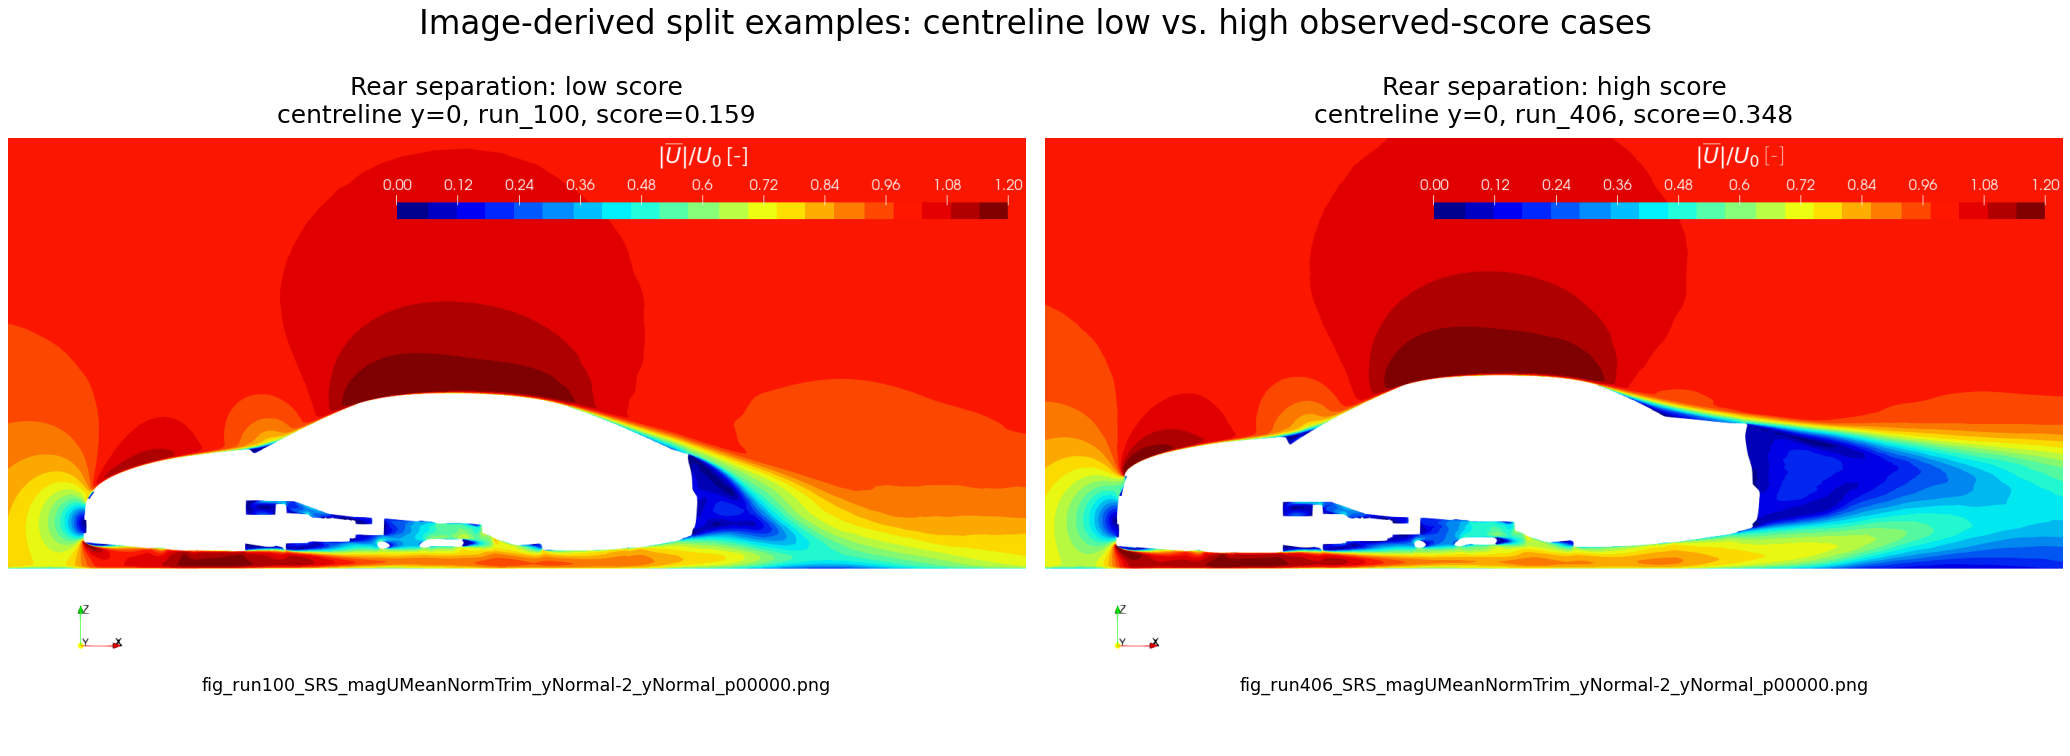
\includegraphics[width=\textwidth]{image_split_examples.png}
  \caption{Centreline velocity-magnitude examples for low and high rear-separation scores. The low-score case is \splitkey{run\_100} (\code{Cd=0.292211}, \code{Cl=0.147656}), and the high-score case is \splitkey{run\_406} (\code{Cd=0.266587}, \code{Cl=0.019273}).}
  \label{fig:image_examples}
\end{figure}

\section*{Repeatability and transparency}

The committed manifest is intended for normal use. The commands below are for
auditing the split construction, recreating the figures, or refreshing the
artifacts after changing the source data.

From a clean split-package checkout, download \code{force\_mom\_all.csv} and
\code{geo\_parameters\_all.csv} from the Hugging Face dataset repo and then
regenerate the manifest and diagnostic plots:

\begin{verbatim}
python3 scripts/download_hf_inputs.py --output-dir data
python3 scripts/generate_splits.py
python3 scripts/visualize_flow_regimes.py
python3 scripts/visualize_image_regimes.py
\end{verbatim}

This exact path uses committed Chamfer geometry scores and committed
rear-separation image scores. To render the example figures from source PNGs
rather than placeholders, also run:

\begin{verbatim}
python3 scripts/download_hf_inputs.py --output-dir data --include-report-images
python3 scripts/visualize_geometry_examples.py
python3 scripts/visualize_split_examples.py
\end{verbatim}

Full report regeneration then uses:

\begin{verbatim}
python3 scripts/generate_splits.py
python3 scripts/visualize_flow_regimes.py
python3 scripts/visualize_geometry_examples.py
python3 scripts/visualize_image_regimes.py
python3 scripts/visualize_split_examples.py
latexmk -pdf -cd docs/README.tex
\end{verbatim}

For an existing dataset checkout, set \code{DRIVAERML\_DATA\_ROOT} to the
directory containing \code{force\_mom\_all.csv} and
\code{geo\_parameters\_all.csv}. If the PNGs live elsewhere, set
\code{DRIVAERML\_IMAGE\_ROOT} to the directory containing
\code{run\_*/images/}.

To recompute \code{data/image\_metrics.csv} from source images, use:

\begin{verbatim}
python3 scripts/download_hf_inputs.py --output-dir data --include-image-score-pngs
python3 scripts/generate_splits.py
\end{verbatim}

To recompute the Chamfer source data from STL meshes, run the standalone
surface-distance script in a work directory and refresh only the metrics CSV
used by the split generator:

\begin{verbatim}
python3 scripts/download_hf_inputs.py --output-dir /tmp/drivaerml_inputs --include-stls
mkdir -p /tmp/drivaerml_chamfer
python3 scripts/compute_chamfer_splits.py \
  --data-root /tmp/drivaerml_inputs \
  --output-dir /tmp/drivaerml_chamfer \
  --samples 10000 \
  --workers 16 \
  --base-manifest splits/manifest.json
cp /tmp/drivaerml_chamfer/chamfer_metrics.csv data/chamfer_metrics.csv
\end{verbatim}

The committed source artifacts were generated against a local checkout with:

\begin{verbatim}
<dataset-root>/force_mom_all.csv
<dataset-root>/geo_parameters_all.csv
<split-package-root>/data/chamfer_metrics.csv
<split-package-root>/splits/manifest.json
<image-root>/run_*/images/
\end{verbatim}

\section*{Manifest format}

\begin{verbatim}
{
    "full_train": ["run_1", "run_2", "..."],
    "full_val": ["run_4", "..."],
    "full_test": ["run_11", "..."],
    "scarce_train": ["run_10", "..."]
}
\end{verbatim}

Case IDs match on-disk directory names and are sorted numerically by run number.

\begin{thebibliography}{9}
\bibitem{drivaerml_dataset}
DrivAerML dataset. \url{https://huggingface.co/datasets/neashton/drivaerml}.

\bibitem{drivaerml_paper}
DrivAerML paper. \url{https://arxiv.org/abs/2408.11969}.

\bibitem{noether_split}
Noether DrivAerML split. \url{https://github.com/Emmi-AI/noether/blob/main/src/noether/data/datasets/cfd/caeml/drivaerml/split.py}.

\bibitem{physicsnemo_loader}
PhysicsNeMo DrivAerNet/DrivAerML-style split loader.
\url{https://docs.nvidia.com/deeplearning/physicsnemo/physicsnemo-core/_modules/physicsnemo/datapipes/gnn/drivaernet_dataset.html}.
\end{thebibliography}

\end{document}
